\section{Previous Findings}

\todo[inline]{
Reorganize: Intro, Relwork, Background, Previous findings?

Relwork:
- Data collections of human user behavior
- Models of human behavior
- - Missing for WCA
- - EdgeDroid 1.0
- Benchmarking of WCA


Validation: train/test split

EdgeDroid 1.0 just shows up in the numerical results.
One paragraph discussing.

}

In~\cite{olguinmunoz2021impact} we studied the effects of system responsiveness on human behavior in step-based \ac{WCA} in a controlled experiment.
We employed a modified and instrumented version of the above-mentioned, step-based LEGO \ac{WCA}~\cite{chen2015early}.
\num{40} subjects interacted with the assistant, performing a \num{169}-step task while we altered the responsiveness in realtime and captured key application and task performance metrics.
Additionally, we also employed questionnaires to evaluate personality traits of the participants, and correlated these results with the task performance metrics.

We used \emph{delay} and execution time as the variables for system responsiveness and human behavior, respectively.
\emph{Delay} corresponded to a temporarily fixed time duration for the processing interval of each frame.
That is, if during a series of steps delay was set to \( D \) seconds, the feedback for each frame was provided to the user \( D \) seconds after frame capture.
The correlation between this variable and execution time was then studied.
To compensate for the distribution of \( t_c \)\footnote{\( t_c \), and conversely the wait time \( \mathcal{W} \) of a step, can be assumed to be uniformly distributed in the interval \( [t_{n - 1}, t_n] \) without loss of generality.}~\cite{olguinmunoz2021impact}, in the present work we adjust the nominal delay \( D \) by a factor \num{1.5}.
We will refer to this adjusted delay as \emph{\acf{TTF}}.

% Delay, however, was merely an experimental tool, and if we consider
% \begin{enumerate*}[itemjoin={{; }}, itemjoin={{; and }}]
%     \item that \( t_c \), and conversely the wait time \( \mathcal{W} \) of a step, can be assumed to be uniformly distributed in the interval \( [t_{n - 1}, t_n] \) without loss of generality~\cite{olguinmunoz:impact2021}
%     \item that for a step subject to delay \( D \), \( t_k - t_{k - 1} = D \) for all \( k \in \{1, 2, \ldots, n\} \)
% \end{enumerate*},
% then it follows that the expected \ac{TTF} for steps subject to a delay \( D \) can be expressed as

% \begin{align}
%     \mathbb{E}\left[\text{\ac{TTF}}\right] &= \mathbb{E}\left[\mathcal{W}\right] + D
%     = \mathbb{E}\left[U(t_{n - 1}, t_n)\right] + D\nonumber\\
%     &= \mathbb{E}\left[U(0, D)\right] + D
%     = \frac{1}{2}D + D = \frac{3}{2}D\label{eq:ttf}
% \end{align}

% Ergo, we can directly re-parameterize the data from~\cite{olguinmunoz:impact2021} to use \ac{TTF} instead of delay by simply multiplying the delay value of each step by \num{1.5}.

Our findings can be summarized as follows:
\begin{enumerate}
    \item System slow-down induces \emph{additional} behavioral slow-down which scales with the decrease in system responsiveness.
    Compared to the unimpaired case, participants were on average \SI{12}{\percent} slower when subject to a mean \ac{TTF} of \SI{2.475}{\second}, and \num{26} percentage points slower at a mean \ac{TTF} of \SI{4.5}{\second}.

    \item\label{item:speedup} At lower \acp{TTF}, humans get faster at performing steps as the task progresses, 
    For sequences of \num{12} steps in an unimpaired application state, humans executed the final four steps on average \SI{36}{\percent} faster than they did the first four.
    However, this effect is dampened by reduced system responsiveness, and actually inverts at the highest levels of system impairment; humans actually become progressively slower the longer they spend in a degraded system state.

    \item\label{item:remain} The effects of system slow-down on human behavior remain for a while even after system responsiveness improves.
    These effects are noticeable for at least \num{4} steps after the return to a high-responsiveness state. 
    
    \item The above effects are modulated by measures of individual levels of personality characteristics and focus.
    % We will discuss this in detail below in \cref{ssec:moderationeffects}
\end{enumerate}

\subsubsection{Moderation of effects by individual characteristics}\label{ssec:moderationeffects}

We recorded variables related to well-known individual differences, encompassing both the \acf{BFI}~\cite{john1999big}, and the \acf{ITQ}~\cite{witmer1998measuring}.
Out of the individual-difference variables, the most salient effect on performance corresponded to \emph{neuroticism}, a \ac{BFI} trait linked to low tolerance for stress and high emotional reactivity, and which has previously been linked to higher \emph{delay discounting} rates~\cite{hirsh2008delay}.
Delay discounting is the tendency to devalue rewards for which one must wait; high rates, indicative of waiting intolerance, have been associated with negative social and academic outcomes.

% Bobby suggested we remove this figure and just give the pearson coeff.
% \begin{figure}
%     \centering
%     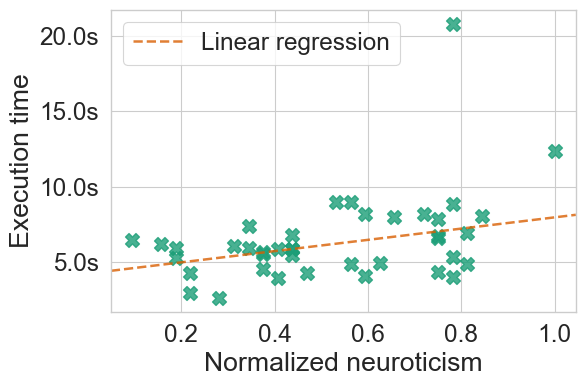
\includegraphics[width=\columnwidth]{figs/new_model/correlation_neuro_exectime.png}
%     \caption{%
%         Correlation between neuroticism and the mean execution time of the last four steps in segments of \num{12} steps subject to the same \ac{TTF} in~\textcite{olguinmunoz:impact2021}.
%         Pearson correlation coefficient \( \rho = 0.418 \), 2-tailed \( p < 0.05 \).
%     }\label{fig:neuroexectimecorrel}
% \end{figure}

In this work, we will use a normalized scale to describe neuroticism, derived from the minimum and maximum obtainable values for this variable in the \ac{BFI}~\cite{john1999big}.
\emph{Low} and \emph{high} neuroticism will refer to the \( [0.0, 0.5) \) and \( [0.5, 1.0] \) ranges respectively.

Linear regression showed a significant correlation between individual neuroticism scores and the execution time late in a series of high-delay steps, \( \rho = 0.418 \), \num{2}-tailed \( p < 0.05 \)
Neuroticism was further identified as a modulating factor for the pacing effects through a \ac{PCA}.
Out of the three identified components, which cumulatively accounted for \SI{73.13}{\percent} of the variance in the results, neuroticism was included in the first two.
The effect of neuroticism was observed across all \acp{TTF} and impairment durations in the tasks.  


\begin{figure}
    \centering
    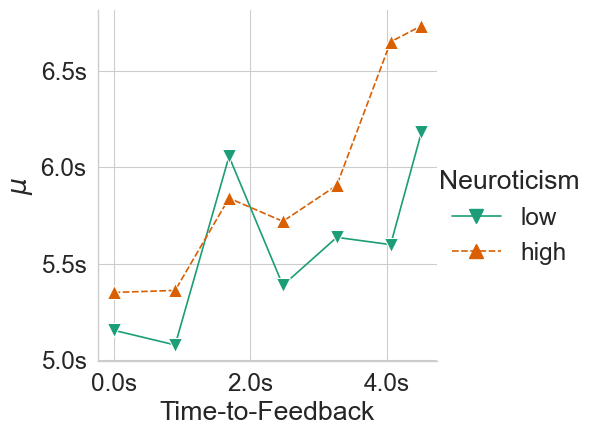
\includegraphics[width=\columnwidth]{figs/new_model/mu_fits_exgaussian_slice0.png}
    \caption{%
        \( \mu \) parameter of \acs*{exGaussian} distributions fitted to execution times of the first four steps of segments of steps subject to the same \ac{TTF} in~\cite{olguinmunoz2021impact}.
        Distributions were fitted using \ac{MLE}.
    }\label{fig:muexgaussian}
\end{figure}

\begin{figure}
    \centering
    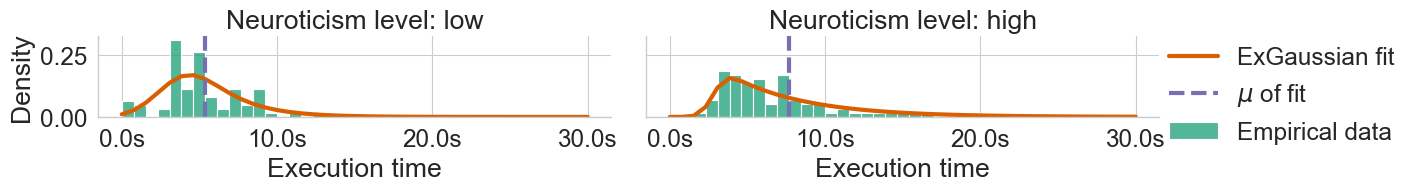
\includegraphics[width=\columnwidth]{figs/new_model/dist_fits_neuro.png}
    \caption{%
        Example \ac{exGaussian} fits on execution times from steps \numrange{4}{8} in a segment of steps at the maximum experimental \ac{TTF}.
        The effects of neuroticism are clearly visible in the tail and the mean of the distributions.
    }\label{fig:fitsneuro}
\end{figure}

Furthermore, we found that execution times, when grouped by experimental variables such as neuroticism, \ac{TTF}, and continuous segments of steps subject to the same \ac{TTF}, were well-fit by an \ac{exGaussian} distribution, as verified using Kolmogorov-Smirnov goodness-of-fit tests~\cite{massey_jr1951kolmogorov}.
When grouping by level of neuroticism, \ac{TTF}, and \emph{slice}\footnote{%
In~\cite{olguinmunoz2021impact} the \emph{slice} to which a step belongs to refers to whether the step occurred in the first, second, or third four-step segment of a sequence of steps subject to the same \ac{TTF}.
}, the best fit statistic was \ensuremath{0.028} (\ensuremath{p = 0.999}).
This distribution has an ample body of research supporting its suitability for the modeling of the timing of human actions and reaction times~\cite{rohrer1994analysis,palmer2011what,marmolejo_ramos2022generalised}.
We found that the effects of neuroticism on execution times were clearly identifiable in the fitted distributions, in particular in their means and tails.
\cref{fig:muexgaussian} shows an example of this modulating effect, illustrating the behavior of the mean (\( \mu \) parameter) of \ac{exGaussian} distributions fitted to the execution times of the first four steps of segments of steps subject to the same \ac{TTF}.
Finally, \cref{fig:fitsneuro} shows an example of the effects of neuroticism on the fitted \ac{exGaussian} distributions for a specific group of execution times.
Higher neuroticism directly translates into a higher mean and longer tail.